\setchapterpreamble[u]{\margintoc}
\chapter{The Artificial Intelligence Industrial Complex}
\labch{introduction}

\textit{"There was a time when everyone thought the quants had figured it out. That is not the perception today. When it comes to the stockmarket, at least, automation has not been the winner-takes-all event that many fear elsewhere. It is more like a tug-of-war between humans and machines. And though the machines are winning, humans have not let go just yet. "} "Lessons from finance's experience with artificial intelligence" The Economist, Mar 9th 2023 \cite{finaieconomist}


\section{The AI Renaissance}

Technology often finds its first adopters among those who can afford it and foresee its potential. Artificial Intelligence (AI) is no exception, with its early applications dating back several decades, notably in the financial industry. Hedge funds and investment banks identified the immense value of AI and started using it for trading and portfolio management.

Renaissance Technologies, a hedge fund founded by mathematician James Simons, exemplifies the early adoption of AI. Since the 1980s, the company has used AI to predict market movements and optimize trading strategies. By employing highly skilled PhDs known as "quants" to develop algorithms and AI models, Renaissance Technologies has become one of the most successful hedge funds in history.

As AI gained traction, tech giants like Google and Microsoft began investing in their own quants. These experts were tasked with using AI to address a wide range of challenges, from refining search algorithms to enhancing language processing capabilities. Much of this research was made public, allowing the broader community to benefit from these advancements.

AI has had a transformative effect on the advertising industry as well. Algorithms now analyze user behavior and target ads with remarkable precision. This has led to an increased demand for privacy-conscious products and services. For example, I carry a Faraday cage fanny pack from a company called "Mission Darkness" to avoid being tracked when I don't want to be. It's a modern-day solution for shielding against unwanted surveillance and data collection.

The accessibility of AI technology has increased, thanks in part to open-source projects that enable individuals and smaller organizations to tap into its power. This democratization of AI has ignited a wave of innovation, with developers worldwide contributing to the AI renaissance.

However, the ubiquity of AI raises some pressing concerns. In a world where data is valuable, the phrase "information wants to be free" takes on new significance. As AI models become more valuable, the risks of data theft and unauthorized sharing escalate. Companies and individuals are striving to protect their intellectual property while others look for ways to exploit it.

This situation sets the stage for an AI copyright battle looming on the horizon. As the distinction between proprietary and open-source information blurs, the question of who owns AI-generated content becomes increasingly important. Governments, corporations, and individuals are all grappling with the legal and ethical implications of AI and its widespread adoption.

So, the AI renaissance has brought about significant advancements in technology, transforming industries and reshaping our world. From the early days of hedge funds like Renaissance Technologies to the current era of open-source AI projects, the landscape has evolved rapidly. As AI continues to permeate our lives, the challenges of data ownership and privacy will become even more critical. In the coming years, we can expect new AI-powered innovations, but also new debates and conflicts as society grapples with the implications of this powerful technology.

\sidecite{copyrighteconocmist}

\section{AI Shrinks the Market, but Takes 80\% Market Share}

The "Software Paradox" posits that as software becomes more valuable, it tends to shrink markets while capturing most of the market share. This phenomenon can be observed in the current state of AI, particularly with the advent of open-source AI. As AI technologies become more sophisticated and widespread, they are reducing the need for human labor in many markets, while simultaneously capturing a significant portion of the market share.\sidecite{OGrady2015}

One key aspect of AI's impact on the market is its ability to automate repetitive and mundane tasks, allowing humans to focus on more complex and creative aspects of their work. This not only streamlines processes but also has the potential to improve the overall quality of work. With AI handling the less desirable tasks, human workers can concentrate on utilizing their unique skills and expertise, resulting in better outcomes and higher value-added work.

The rise of open-source AI further accelerates this trend, making advanced AI tools and algorithms accessible to a broader range of individuals and organizations. As these powerful tools become more widely available, businesses across various industries will find it increasingly difficult to justify the cost of employing human workers for tasks that can be more efficiently completed by AI. This shift will result in a smaller job market for those specific tasks, with AI taking the majority of the market share.

However, the shrinking of specific labor markets does not necessarily mean the eradication of all human work. Instead, it presents an opportunity for the workforce to adapt and focus on roles that are complementary to AI systems. This could involve tasks that require empathy, complex problem-solving, or human intuition, which are areas where AI currently struggles to excel.

\section{The Other Economy, the One Without AI}

As AI revolutionizes various sectors of the economy, there's another economy that remains untouched by AI's transformative effects. This other economy is characterized by heavily regulated industries that often resist technological innovation, resulting in stagnating growth and rising costs for consumers\sidecite{andreesenunemp}.

In many places, AI is practically illegal. This is partly due to consumers, professional organizations and governments struggling to keep up with the rapid pace of technological advancements, leading to a lack of understanding and appropriate regulations \sidecite{lawmakersny}. Additionally, public opinion remains skeptical about the widespread adoption of AI, as evidenced by polls\sidecite{morningconsult}\sidecite{monmouthai}. This skepticism is not helped by stories of software developers becoming emotionally attached to AI chatbots\sidecite{googlenerd}.

The contrast between sectors that embrace AI and those that resist it highlights a growing divide in the economy. In industries where AI is allowed to flourish, technological innovation drives down prices and increases product quality, leading to a more efficient market. However, heavily regulated sectors that resist AI adoption experience rising costs and stagnating growth, ultimately consuming a larger share of the economy.

This phenomenon is exacerbated by the emotional interplay between production and consumption. As consumers, we tend to become frustrated with price increases in the heavily regulated sectors. On the other hand, as producers, we may feel threatened by technological disruption in industries that embrace AI. This dichotomy demonstrates the inherent conflict between the desire for stability in the economy and the need for innovation and progress.

As the regulated, non-technological sectors continue to grow as a percentage of GDP, the economy may ultimately become dominated by these stagnating industries. In such a scenario, the full potential of AI and other advanced technologies may never be realized. This highlights the importance of addressing regulatory barriers, fostering public understanding, and promoting AI adoption in industries that have yet to embrace its potential.

The existence of an economy without AI underscores the challenges that lie ahead in integrating advanced technologies into every aspect of our lives. To fully realize the benefits of AI, it is crucial to address the legal, regulatory, and public perception barriers that currently hinder its adoption. By doing so, we can work towards a more efficient and innovative economy that harnesses the power of AI for the benefit of all.


\section{(Human and AI) Workers of The World, Unite!}

AI's adoption can be seen as an extension of the outsourcing trend that has been prevalent for decades. The principle "if you can't beat them, join them" seems more relevant than ever, as people increasingly integrate AI into their work and lives.

Even in places where AI is technically illegal or frowned upon, individuals find creative ways to leverage AI to make their lives easier. Students may use AI to help write essays, office workers may employ Optical Character Recognition (OCR) to avoid tedious data entry tasks, and programmers might utilize GitHub Copilot regardless of whether their employers approve. These examples demonstrate that as AI tools become more accessible and affordable, they will infiltrate various industries.

\begin{marginfigure}[-5.5cm]
    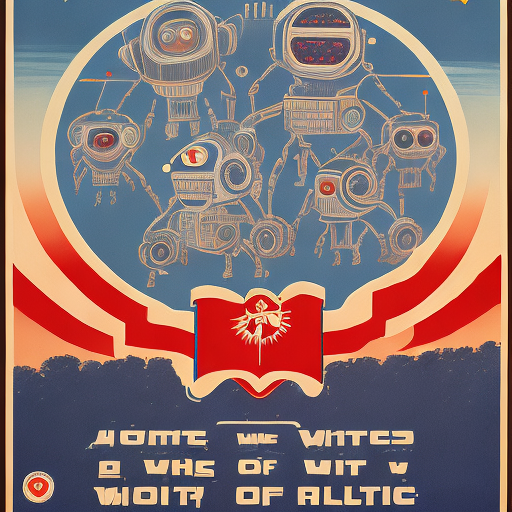
\includegraphics{unite}
        \caption{"mdjrny-v4 style a propaganda poster that says 'AI and Human Workers of the World Unite' featuring some robots and humans laboring together in the fields, USSR-style 8k" made with Mann-E}
        \labfig{marginunite}
\end{marginfigure}

Instead of resisting this trend, we should work with it and guide its development. Embracing AI and integrating it into our work processes can lead to increased productivity, innovation, and overall improvement in our quality of life\sidecite{peopleusingAIhappy}.

The situation with AI usage is reminiscent of self-driving cars and semi-autonomous driving modes. Despite manufacturers' intentions and guidelines, these features are often treated as fully autonomous by users, reflecting the human tendency to push boundaries and adapt technology to suit their needs.

As AI becomes more ingrained in our daily lives, it's essential to recognize the inevitability of its adoption and focus on guiding its development in a way that maximizes its benefits and minimizes potential risks. By uniting human and AI workers, we can foster a collaborative environment that leverages the strengths of both entities and paves the way for a more efficient, innovative, and prosperous future. \sidecite{protopia}

\section{Is it The Future Yet?}

AI, as a general-purpose technology, has the potential to transform various aspects of our lives. However, its widespread adoption and impact on Total Factor Productivity (TFP) might not happen overnight. History has shown that even groundbreaking general-purpose technologies can take time to reach their full potential.

Take electricity, for example. Although Thomas Edison invented the light bulb in 1879, it took several decades for electricity to become the primary power source in industries and households. The infrastructure required to generate and distribute electricity on a large scale was built gradually, and businesses needed time to adapt their processes and machinery to leverage this new energy source. It wasn't until the early 20th century that the true impact of electricity on productivity and economic growth was realized.

Another example is the steam engine, invented by James Watt in 1775, which marked the beginning of the Industrial Revolution. The technology's full potential was not realized until several decades later. The adoption of steam-powered machinery required significant investments in infrastructure and the reorganization of production processes. Additionally, the development of railway networks and steamships expanded the reach of this technology, leading to a profound impact on productivity and global trade.

The internet also followed a similar pattern. While the internet was conceived in the late 1960s, it wasn't until the 1990s that its commercial potential began to be explored. The widespread adoption of the internet required the development of user-friendly web browsers, the expansion of telecommunications infrastructure, and the emergence of e-commerce platforms. It took several years for the internet to become an integral part of our daily lives and contribute to increased productivity across various industries.

So, while AI has the potential to revolutionize numerous aspects of our lives, it may take time for this technology to fully permeate our society and yield its maximum benefits. Patience and continuous innovation will be essential in realizing the transformative potential of AI. By learning from the history of general-purpose technologies, we can better understand the trajectory AI might follow and work towards a future where it significantly impacts productivity and our everyday lives.

\section{Key Takeaways}

\begin{itemize}
    \item \textbf{Deep learning presents challenges and opportunities}, with the potential to become a powerful, free tool for innovation.\sidenote{The Free Software Foundation's goals align with the inherent nature of deep learning models.}
    \item \textbf{Deep learning can be used as an "employee"} for non-critical tasks, offering a balance between dystopian and utopian visions of the future.\sidenote{Work will transform, and humans will act as supervisors and managers of these new technological workers.}
\end{itemize}
